%%%%%%%%%%%%%%%%%%%%%%%%%%%%%%%%%%%%%%%%%
% Programming/Coding Assignment
% LaTeX Template
%
% This template has been downloaded from:
% http://www.latextemplates.com
%
% Original author:
% Ted Pavlic (http://www.tedpavlic.com)
%
% Note:
% The \lipsum[#] commands throughout this template generate dummy text
% to fill the template out. These commands should all be removed when 
% writing assignment content.
%
% This template uses a Perl script as an example snippet of code, most other
% languages are also usable. Configure them in the "CODE INCLUSION 
% CONFIGURATION" section.
%
%%%%%%%%%%%%%%%%%%%%%%%%%%%%%%%%%%%%%%%%%

%----------------------------------------------------------------------------------------
%	PACKAGES AND OTHER DOCUMENT CONFIGURATIONS
%----------------------------------------------------------------------------------------

\documentclass{article}

\usepackage{fancyhdr} % Required for custom headers
\usepackage{lastpage} % Required to determine the last page for the footer
\usepackage{extramarks} % Required for headers and footers
\usepackage[usenames,dvipsnames]{color} % Required for custom colors
\usepackage{graphicx} % Required to insert images
\usepackage{subcaption}
\usepackage{listings} % Required for insertion of code
\usepackage{courier} % Required for the courier font
\usepackage{amsmath}
\usepackage{lipsum} % Used for inserting dummy 'Lorem ipsum' text into the template

% Margins
\topmargin=-0.45in
\evensidemargin=0in
\oddsidemargin=0in
\textwidth=6.5in
\textheight=9.0in
\headsep=0.25in

\linespread{1.1} % Line spacing

% Set up the header and footer
\pagestyle{fancy}
\lhead{\hmwkAuthorName} % Top left header
\chead{\hmwkClass\ (\hmwkClassTime): \hmwkTitle} % Top center head
%\rhead{\firstxmark} % Top right header
\lfoot{\lastxmark} % Bottom left footer
\cfoot{} % Bottom center footer
\rfoot{Page\ \thepage\ of\ \protect\pageref{LastPage}} % Bottom right footer
\renewcommand\headrulewidth{0.4pt} % Size of the header rule
\renewcommand\footrulewidth{0.4pt} % Size of the footer rule

\setlength\parindent{0pt} % Removes all indentation from paragraphs

%----------------------------------------------------------------------------------------
%	CODE INCLUSION CONFIGURATION
%----------------------------------------------------------------------------------------

\definecolor{MyDarkGreen}{rgb}{0.0,0.4,0.0} % This is the color used for comments
\lstloadlanguages{Perl} % Load Perl syntax for listings, for a list of other languages supported see: ftp://ftp.tex.ac.uk/tex-archive/macros/latex/contrib/listings/listings.pdf
\lstset{language=Perl, % Use Perl in this example
        frame=single, % Single frame around code
        basicstyle=\small\ttfamily, % Use small true type font
        keywordstyle=[1]\color{Blue}\bf, % Perl functions bold and blue
        keywordstyle=[2]\color{Purple}, % Perl function arguments purple
        keywordstyle=[3]\color{Blue}\underbar, % Custom functions underlined and blue
        identifierstyle=, % Nothing special about identifiers                                         
        commentstyle=\usefont{T1}{pcr}{m}{sl}\color{MyDarkGreen}\small, % Comments small dark green courier font
        stringstyle=\color{Purple}, % Strings are purple
        showstringspaces=false, % Don't put marks in string spaces
        tabsize=5, % 5 spaces per tab
        %
        % Put standard Perl functions not included in the default language here
        morekeywords={rand},
        %
        % Put Perl function parameters here
        morekeywords=[2]{on, off, interp},
        %
        % Put user defined functions here
        morekeywords=[3]{test},
       	%
        morecomment=[l][\color{Blue}]{...}, % Line continuation (...) like blue comment
        numbers=left, % Line numbers on left
        firstnumber=1, % Line numbers start with line 1
        numberstyle=\tiny\color{Blue}, % Line numbers are blue and small
        stepnumber=5 % Line numbers go in steps of 5
}

% Creates a new command to include a perl script, the first parameter is the filename of the script (without .pl), the second parameter is the caption
\newcommand{\perlscript}[2]{
\begin{itemize}
\item[]\lstinputlisting[caption=#2,label=#1]{#1.pl}
\end{itemize}
}

%----------------------------------------------------------------------------------------
%	DOCUMENT STRUCTURE COMMANDS
%	Skip this unless you know what you're doing
%----------------------------------------------------------------------------------------

% Header and footer for when a page split occurs within a problem environment
\newcommand{\enterProblemHeader}[1]{
%\nobreak\extramarks{#1}{#1 continued on next page\ldots}\nobreak
%\nobreak\extramarks{#1 (continued)}{#1 continued on next page\ldots}\nobreak
}

% Header and footer for when a page split occurs between problem environments
\newcommand{\exitProblemHeader}[1]{
%\nobreak\extramarks{#1 (continued)}{#1 continued on next page\ldots}\nobreak
%\nobreak\extramarks{#1}{}\nobreak
}

\setcounter{secnumdepth}{0} % Removes default section numbers
\newcounter{homeworkProblemCounter} % Creates a counter to keep track of the number of problems
\setcounter{homeworkProblemCounter}{0}

\newcommand{\homeworkProblemName}{}
\newenvironment{homeworkProblem}[1][Problem \arabic{homeworkProblemCounter}]{ % Makes a new environment called homeworkProblem which takes 1 argument (custom name) but the default is "Problem #"
\stepcounter{homeworkProblemCounter} % Increase counter for number of problems
\renewcommand{\homeworkProblemName}{#1} % Assign \homeworkProblemName the name of the problem
\section{\homeworkProblemName} % Make a section in the document with the custom problem count
\enterProblemHeader{\homeworkProblemName} % Header and footer within the environment
}{
\exitProblemHeader{\homeworkProblemName} % Header and footer after the environment
}

\newcommand{\problemAnswer}[1]{ % Defines the problem answer command with the content as the only argument
\noindent\framebox[\columnwidth][c]{\begin{minipage}{0.98\columnwidth}#1\end{minipage}} % Makes the box around the problem answer and puts the content inside
}

\newcommand{\homeworkSectionName}{}
\newenvironment{homeworkSection}[1]{ % New environment for sections within homework problems, takes 1 argument - the name of the section
\renewcommand{\homeworkSectionName}{#1} % Assign \homeworkSectionName to the name of the section from the environment argument
\subsection{\homeworkSectionName} % Make a subsection with the custom name of the subsection
\enterProblemHeader{\homeworkProblemName\ [\homeworkSectionName]} % Header and footer within the environment
}{
\enterProblemHeader{\homeworkProblemName} % Header and footer after the environment
}

%----------------------------------------------------------------------------------------
%	NAME AND CLASS SECTION
%----------------------------------------------------------------------------------------

\newcommand{\hmwkTitle}{Assignment\ \#$\sqrt{1}$} % Assignment title
\newcommand{\hmwkDueDate}{Sunday,\ January\ 29,\ 2017} % Due date
\newcommand{\hmwkClass}{CSC411} % Course/class
\newcommand{\hmwkClassTime}{L0101} % Class/lecture time
\newcommand{\hmwkAuthorName}{Naireen Hussain} % Your name

%----------------------------------------------------------------------------------------
%	TITLE PAGE
%----------------------------------------------------------------------------------------

\title{
\vspace{2in}
\textmd{\textbf{\hmwkClass:\ \hmwkTitle}}\\
\normalsize\vspace{0.1in}\small{Due\ on\ \hmwkDueDate}\\
\vspace{0.1in}
\vspace{3in}
}

\author{\textbf{\hmwkAuthorName}}
%\date{} % Insert date here if you want it to appear below your name

%----------------------------------------------------------------------------------------

\begin{document}

\maketitle
\clearpage
%----------------------------------------------------------------------------------------
%	PROBLEM 1
%----------------------------------------------------------------------------------------

% To have just one problem per page, simply put a \clearpage after each problem

\begin{homeworkProblem}

\noindent \textit{Part 1: Describing the Data}

The collection of data is quite poorly maintained as there were several URL links that were no longer valid. For some cases, the image had been removed, and replaced with another image, as shown below. These images were not removed.  Afterwards, I cropped the images, but there were quite a few where the bounding box extended outside of the actual image, so there were only 1273 left for the 6 actors from the original 1397. The way the invalid bounds were handled were that those images were completely ignored. There were enough images that this was a viable option.  Furthermore, while some bounding boxes were accurate in capturing the face,  there were some that were not. Some were so inaccurate that one photo had two people, and the bounding box bounded the wrong face, as seen in Figure \ref{fig:pic_qual}. Other times, part of the face would be cut off, like the chin or the forehead, and in other cases, the bounding box missed the face entirely. No poorly bounded data was removed.  All images shown below are after they have been cropped by the bounding box, and before they have been re-sized and recolored.

Here are some that were not correctly bounded, or had other issues:

\begin{figure}[h]

\includegraphics[width=.3\textwidth]{pics/carell176.jpg}\hfill
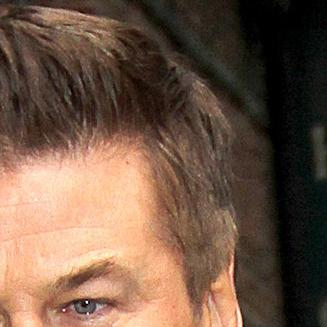
\includegraphics[width=.3\textwidth]{pics/baldwin16.jpg}\hfill

\includegraphics[width=.3\textwidth]{pics/carell21.jpg}
\caption{The first image to the left had its image replaced. The middle picture had an incorrect bounding box, so only part of the face was captured. The last one did have a good bounding box, but got the wrong face, as this was supposed to be Steve Carell. \label{fig:pic_qual}}
\end{figure}

Here are some that were bounded correctly:

\begin{figure}[h]
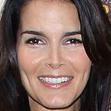
\includegraphics[width=.3\textwidth]{pics/harmon133.jpg}\hfill

\includegraphics[width=.3\textwidth]{pics/gilpin94.jpg}\hfill
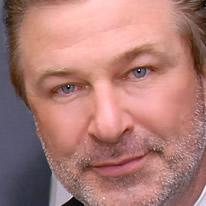
\includegraphics[width=.3\textwidth]{pics/baldwin7.jpg}
\caption{These images were bounded correctly. Even though they all depict a face, they aren't all alighed, since the actors a in a variety of different poses. These pictures also have a tiny bit of either the forehead or the chin cut off. \label{fig:good_box}}
\end{figure}

Many of these images don't have their faces aligned, since the actors weren't all in the same pose when these photos were taken. In Figure \ref{fig:good_box}, the middle actress has here face slightly turned away from the camera, and the right actor has his head slightly tilted.

Here are some pictures that haven't been cropped yet:


\begin{figure}[h]
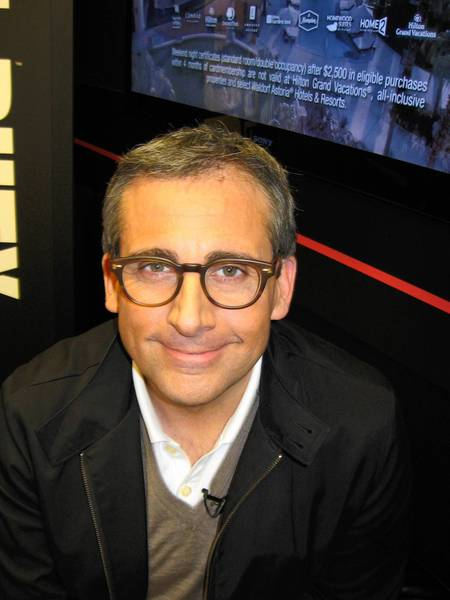
\includegraphics[width=.3\textwidth]{pics/Steve-Carell-Original.jpg}\hfill
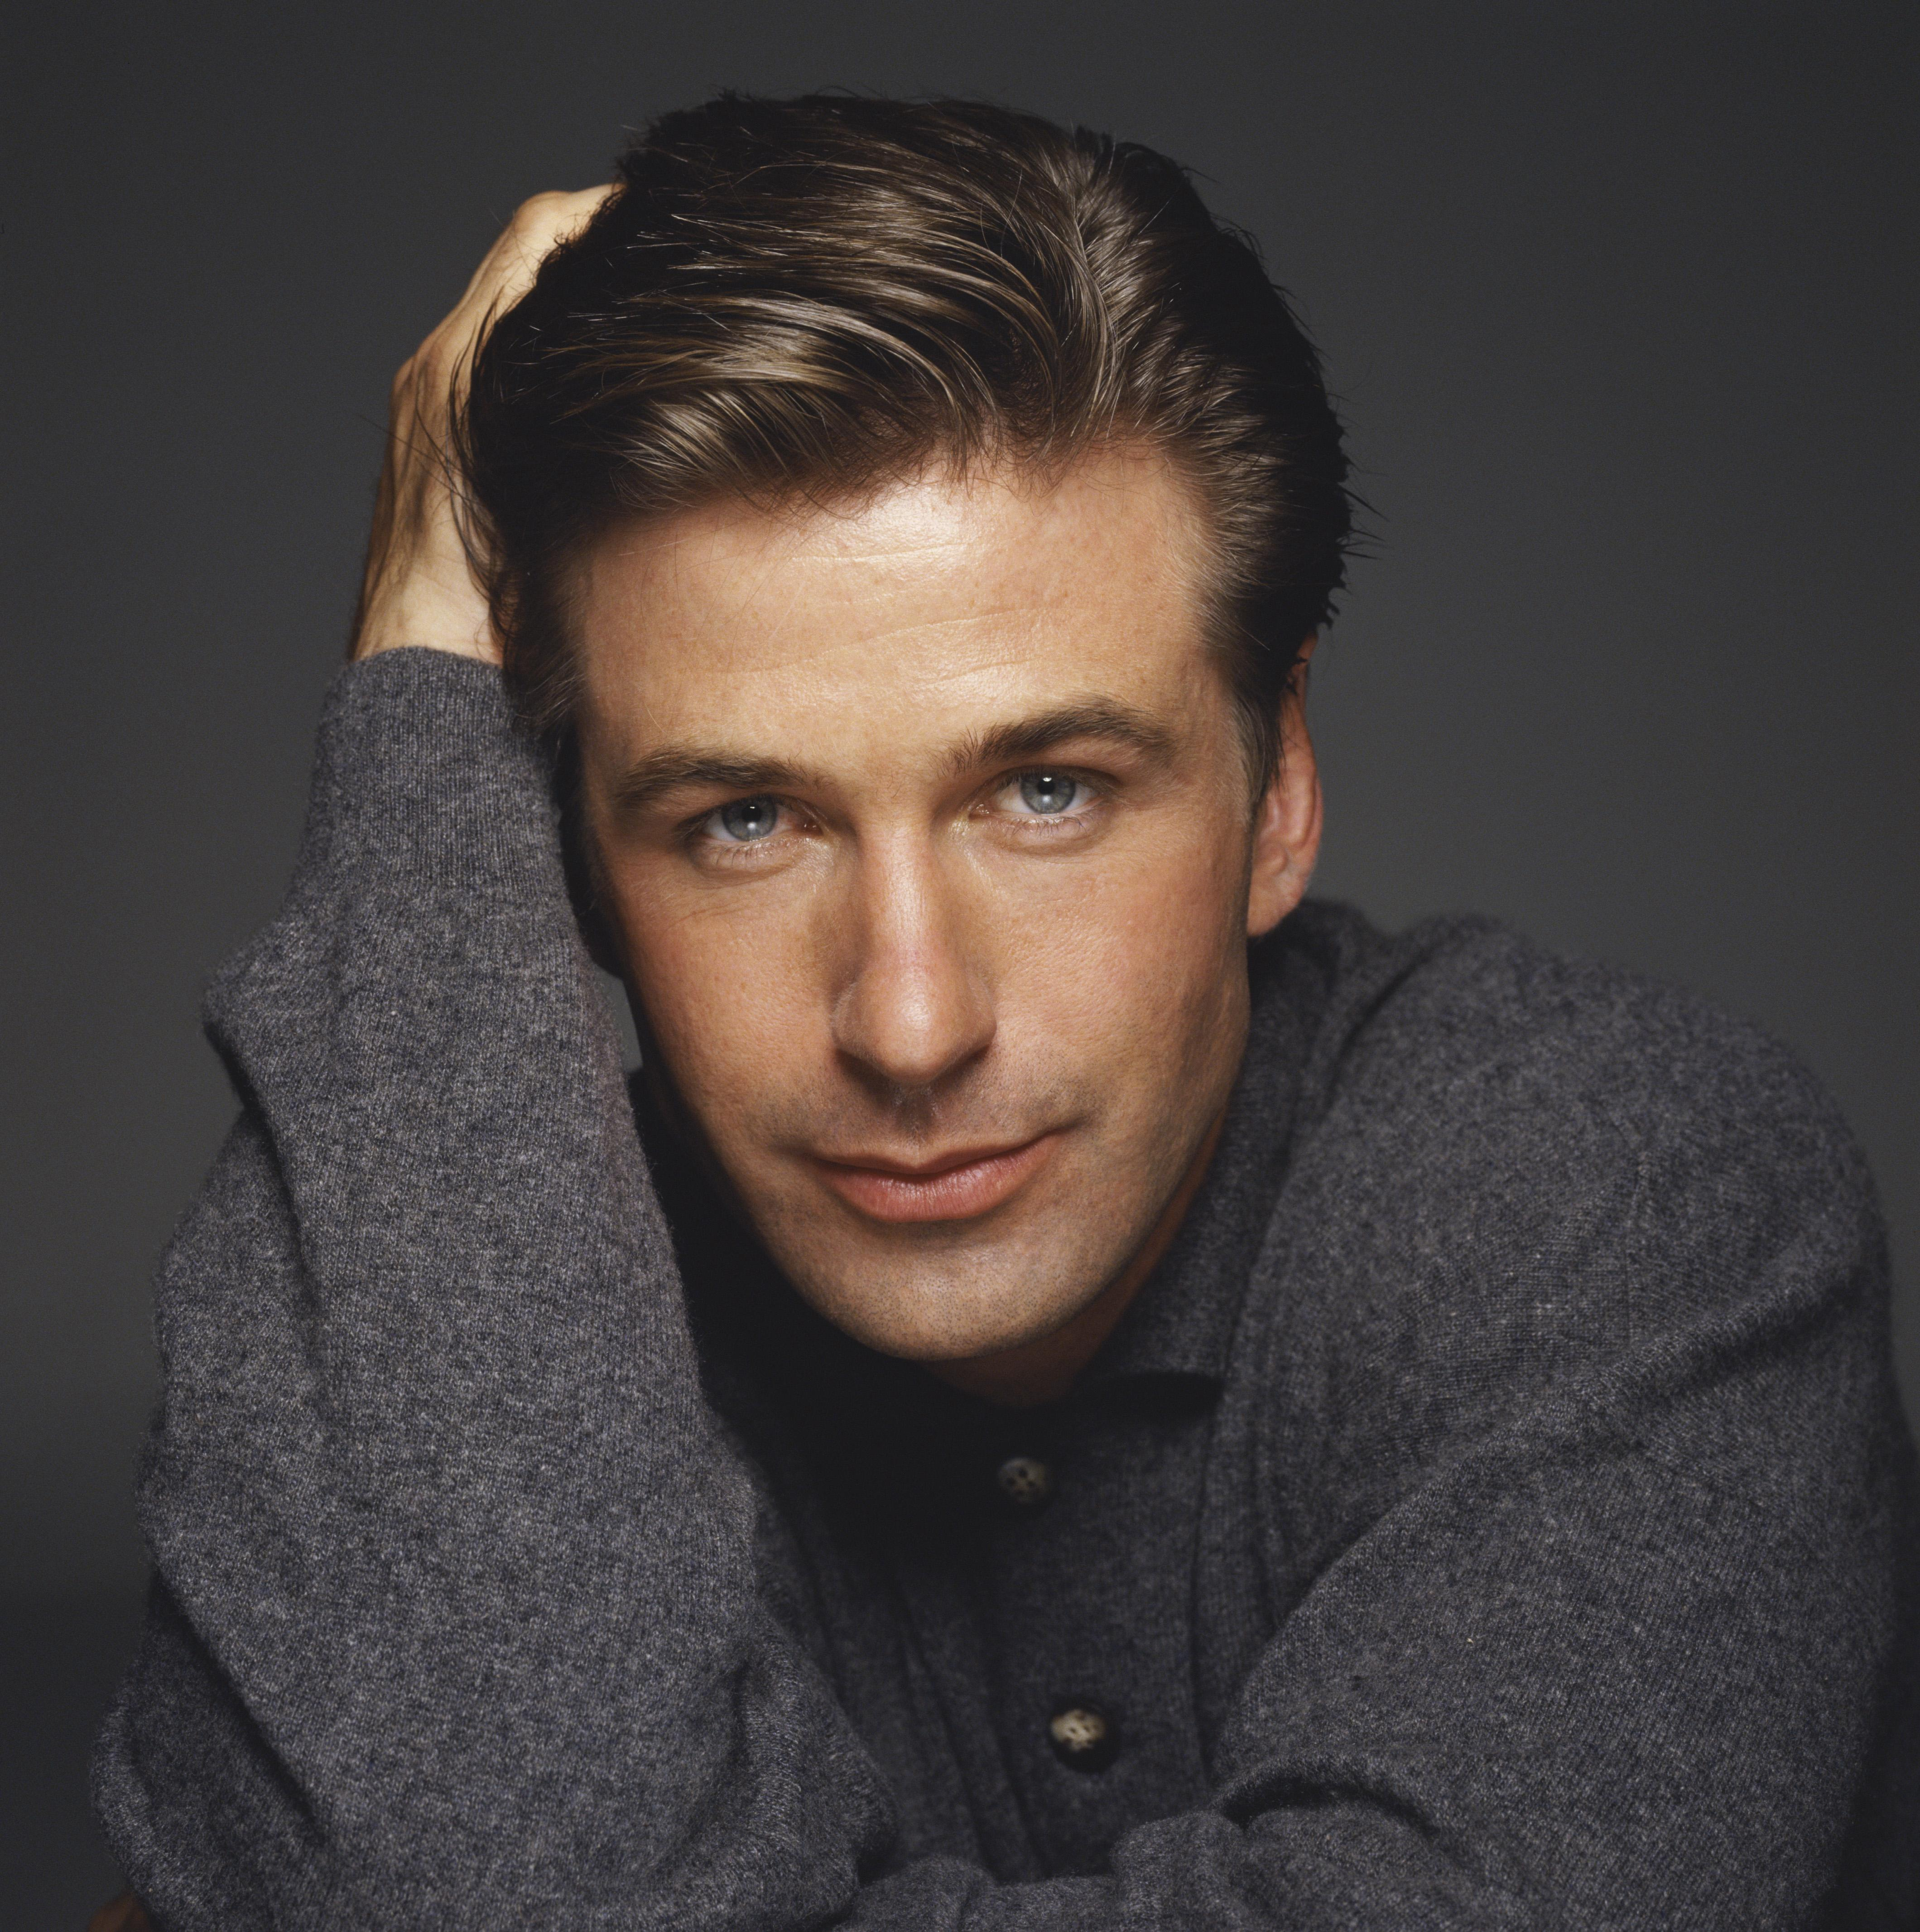
\includegraphics[width=.3\textwidth]{pics/Alec-Baldwin-Original.jpg}\hfill
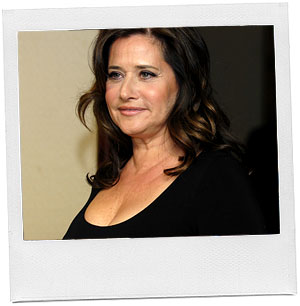
\includegraphics[width=.3\textwidth]{pics/Bracco.jpg}
\caption{These are some images that haven't been bounded yet. \label{fig:orig_box}}
\end{figure}

\end{homeworkProblem}

%\clearpage
%----------------------------------------------------------------------------------------
%	PROBLEM 2
%----------------------------------------------------------------------------------------

\begin{homeworkProblem}
\noindent \textit{Selecting The data}

Working with the cropped data, I collected the first 110 valid images, and designated that as the training set, and then selected the next 10 for validation, and then the next 10 made up the test set. This means that there were a total of 130 valid images per actor. I did not feel the need to shuffle the data, as it seemed like the listing of picture URLS were already random, so there would be no added value in reshuffling the data. Valid images are images that could be successfully opened to ensure that they were not corrupted. Images at this stage were already checked to make sure they were properly cropped, resized and recolored.

Here is code below with the appropriate error handling. This is in file sort\_data2.py 

\begin{lstlisting}
import os
import matplotlib.image as mpimg
import numpy as np
from shutil import copyfile
from matplotlib import pyplot as plt

act = list(set([a.split("\t")[0].replace("\n", "") 
	for a in open("subset_actors.txt").readlines()]))

files = os.listdir("processed/")

print(len(files))
for name in act:
    counter = 0
    for file_name in files:
        if name.split(" ")[1].lower() in file_name:
            #if the actor is in the file name of pic sort the images in approriate spot accordingly
            if counter > 130:
                breaks
            try:
                if counter <110:
                    copyfile("processed/" + file_name, "Train/" + file_name)
                elif counter<120: 
                    copyfile("processed/" + file_name, "Validation/" + file_name)
                elif counter<130:
                    copyfile("processed/" + file_name, "Test/" + file_name)
                counter +=1
                print(counter)
            except Exception as e:
                print(e)
            #once while loop concludes,
            if counter > 130:
                break

\end{lstlisting}


\end{homeworkProblem}
\clearpage
%----------------------------------------------------------------------------------------
%	PROBLEM 3
%----------------------------------------------------------------------------------------



\begin{homeworkProblem}
\noindent \textit{ The Model - Gradient Descent }

I used a linear regression classifier model to classify the images. The images of Alec Baldwin were compared against those of Steve Carell. Baldwin was labelled 0, and Carell was labelled 1. There were 220 images in the training set, and then 20 in the validation set. The model got 214 (97.2\%) correct on the training set, and 13 (65\%) on the validation set. It makes sense that the model does well on the training set, since its predicting on images that were used to construct the model itself. These are results generated when $\Theta$ is initialized as a zero vector for the gradient descent. 

Since the linear regression model returns the dot product of $\Theta^TX$, which is a continuous value, it needs to be mapped to a binary value of either 0 or 1 for binary classification. For any data point that had a score of less than 0.5, it was mapped to 0, and everything above 0.5 was mapped to 1. 


Here is the code to generate the predictions for the validation set after the $\Theta$ vector has been determined through gradient descent. 

The cost function minimized was 

\begin{equation}
J(\Theta_0 , ...\Theta_{1025}) = \sum_{i=1} ^m (h_{\Theta}(x^{(i)}) - y^{(i)}) ^2 
\label{eq:cost1}
\end{equation}


The constants $\frac{1}{2m}$ was dropped as $m$ is constant, so that missing factor is just scales the answer, but the direction of the gradient searched in gradient descent remains unchanged. 

\begin{lstlisting}
#predictions on the validation set, 
preds = np.zeros_like(valid_y)
valid_data_ones = np.concatenate((np.ones((1, valid_data.shape[0])).T, valid_data), 
	axis = 1)
preds = np.dot(valid_data_ones, theta)

#map preds to binary outputs
preds_binary= np.zeros_like(preds)
preds_binary[preds<0.5] = 0
preds_binary[preds>0.5] = 1
#compute how many the model got right
print len(np.where(valid_y ==preds_binary)[0])
\end{lstlisting}


To get the model to work, some fine tuning was required. For example, the model would not work if the learning rate $\alpha $ was too large. Trial and error was used to find a value that worked, and then further tuning was done to find a value that would give a higher score. This was determined to be 1 x$10 ^{-5}$. Another value that I tuned was $\epsilon$, which determines when the model stops. If the change in $\Theta$ is less than $\epsilon$ during one iteration, then gradient descent stops. The larger $\epsilon$ is, the quicker the model stops. This was also manually tuned to an optimal value of 1 x$10^{-4}$. Lastly, a common error I was running into was arithmetic overflow. This occurred when running gradient descent with the original pixel values. To solve this, I scaled down all pixel values by 256. 


Here are the first 10 cost values for the training set:

\begin{lstlisting}
 [0.28289115  0.11183247  0.20492276 -0.00654187  0.10977967  0.13322678
  0.29099036  0.0232449  -0.00654187  0.28450416]
\end{lstlisting}


Here are the first 10 cost values for the training set:

\begin{lstlisting}
 [0.39899181 0.29958775 0.24561934 0.67736738 0.26899213 0.5821788
 0.57735219 0.48045102 0.51039915 0.43317688]
\end{lstlisting}

Here are two distribution plots of the scores

\begin{figure}[h]
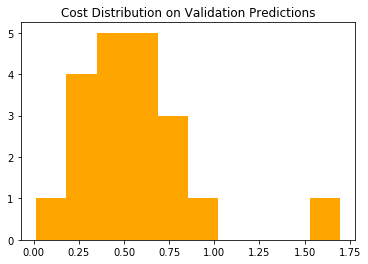
\includegraphics[width=.5\textwidth]{pics/cost_preds.png}\hfill
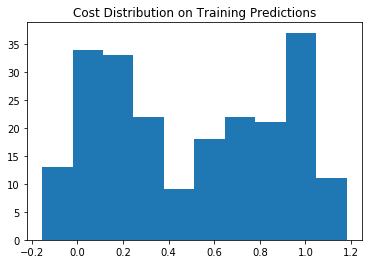
\includegraphics[width=.5\textwidth]{pics/cost_train.png}\hfill
\caption{These are the cost distibutions of bothe the traing. \label{fig:cost_dist}}
\end{figure}

\end{homeworkProblem}
%\clearpage

%----------------------------------------------------------------------------------------
%	PROBLEM 4
%----------------------------------------------------------------------------------------

\begin{homeworkProblem}
\section*{A}
\noindent \textit{Representing Theta}

The model J($\Theta$) can also be visualized. Here is how it looks trained on the full set of 220 images. 


\begin{figure}[h]
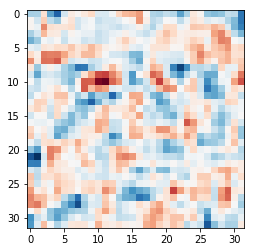
\includegraphics[width=.4\textwidth]{pics/full_zeros.png}\hfill
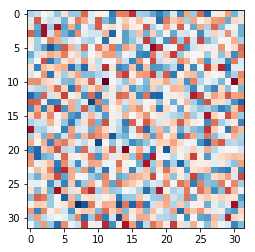
\includegraphics[width=.4\textwidth]{pics/full_random.png}
%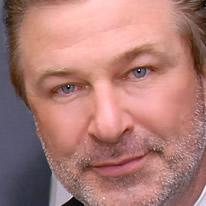
\includegraphics[width=.3\textwidth]{pics/baldwin7.jpg}
\caption{Both images are produced by training on the entire training data set of 220. The left image is produced by initializing $\Theta$ as all zeros, and the second one is done with $\Theta$ initialized with np.random.random, with the random seed set to 0.}
\end{figure}


\begin{figure}[h]
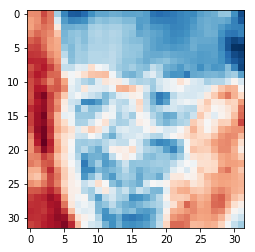
\includegraphics[width=.4\textwidth]{pics/two_zeros.png}\hfill
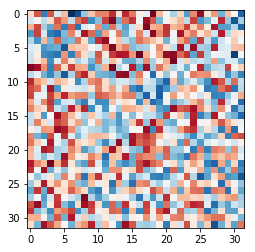
\includegraphics[width=.4\textwidth]{pics/two_random.png}
%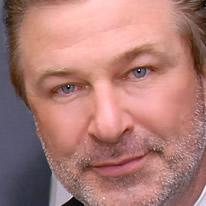
\includegraphics[width=.3\textwidth]{pics/baldwin7.jpg}
\caption{Both images are produced by training on the entire training data set of 220. The left image is produced by initializing $\Theta$ as all zeros, and the second one is done with $\Theta$ initialized with np.random.random, with the random seed set to 0.}
\end{figure}


\section*{B}
Different images can be produced by stopping the gradient descent earlier.


\begin{figure}[h]
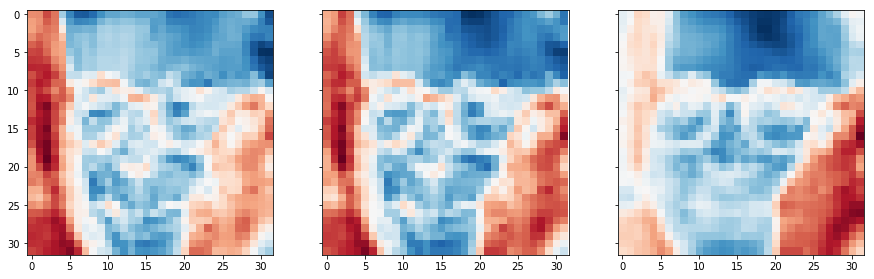
\includegraphics[scale=0.5]{pics/stop_points.png}
\caption{These were generated by tuning the epsilon parameter to stop the gradient descent early. Learning rate values of $10^{-4}, 10^{-5}, 10^{-6}$ , gave 370, 183, and 1 iterations for gradient descent respectively. The images are in that order from left to right. In these runs, $\epsilon$ was kept constant at 1 x$10^{-4}$ The longer the algorithm runs, the more different the visualization of theta looks from an image. This is done on a dataset of 4, with 2 images of Carell and Baldwin each.}

\end{figure}

\end{homeworkProblem}
%\clearpage

%----------------------------------------------------------------------------------------

\begin{homeworkProblem}

\noindent \textit{Gender Classification}

Since there were 110 images collected for each actor, I has 330 female and male pictures for training, and then 30 male and 30 female pictures for validation amd then another set of 30 male and 30 female pictures for as testing. However, for testing, the 60 faces were used were of actors that were not included in the training or validation stage.  The male actors used were Daniel Radcliffe, Gerard Butler and  Micheal Vartan, and the female actors were Kristen Chenoweth, America Ferrera, and Fran Drescher.
The scores noticeably decrease as the training size increases. This is because the model is beginning to learn the noise in the data, which should not translate well to the validation data set. The score does not vary on the test set or the validation set. The model performs slightly better on the test set than the validation set. Sizes of 110, 220, 330, 440, 550 and 660 were used for the training set to determine how the performance would vary.


\begin{figure}[h]
\centering
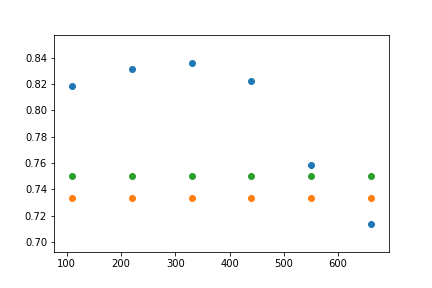
\includegraphics[scale=0.8]{pics/overfitting.png}
\end{figure}




\end{homeworkProblem}



%Q6

\begin{homeworkProblem}
\noindent \textit{Multi-Classification with One Hot Key Encoding}

\section*{A}




\begin{equation}
J(\Theta) = \sum_i^k ( \sum_j^n(\Theta^T_{ij}x^{(i)} -y^{i} )_j^2 )
\end{equation}

%\begin{equation}
%\frac{\partial J}{\partial \Theta_{pq}} =
\[ \frac{\partial J}{\partial \Theta_{pq}} \begin{cases}
 	2x^{i}(\Theta^T_{pq}x^{(i)} -y^{i} )_j, i = p, j = q\\
	0, i \neq p, j \neq q\\
\end{cases}
\]
%\end{eqnarray}

\section*{B}


\begin{equation}
\frac{\partial J}{\partial \Theta_{10}} = 2x^{1}(\Theta^T_{10}x^{(1)} -y^{(1)} )_0\\
\end{equation}

\begin{equation}
\frac{\partial J}{\partial \Theta_{01}} = 2x^{0}(\Theta^T_{01}x^{(0)} -y^{0} )_1\\
\end{equation}

The other derivatives in each of the components will be similar, and are each a scalar. A factor of 2 can be pulled out, and can be rearranged to get the following:

\begin{equation}
\frac{\partial J}{\partial \Theta} =  2X(\Theta^TX -Y)^T
\end{equation}

Here $\Theta$ is an $n$ by $k$ matrix. $k$ is the number of features each sample has, which in this case is 1025. $X$ is an $n$ by $m$ matrix, where $m$ represents the number of samples. Thus, the result of $\Theta^T X$ would be $k$ by $m$ matrix, which matches the dimensions of Y. The final gradient matrix has the dimensions $n$ by $k$, which corresponds to each row being the derivative of the image's performance, and each column corresponds to each individual $\theta$ component.

\section*{C}
Here is the vectorized Cost Function
\begin{lstlisting}
def df(x, y, theta):
    bias = np.ones( (1, x.shape[0]))
    x = np.hstack( (bias.T, x))
    return  2*np.dot(x.T,(np.dot(theta.T, x.T) - y.T).T )
\end{lstlisting}

\section*{D}
To test the gradient, I used the method of finite differences. I used an h value of $1^{-5}$. This is because this was enough to have the first 6 significant digits match for the derivatives computed with this method and with gradient descent for 4 of the 5 tested components. The first test component differed quite a bit. I used the $\Theta$ vector computed during gradient descent.


\begin{lstlisting}
# Finite Difference checks, 5 elements
h = 0.00001
for i in range(5):
    test_theta_h =  theta.copy()
    test_theta_h[i, 0] += h
    print ((f(train_data, train_y, test_theta_h ) - f(train_data, train_y, theta))/(h))
    print df(train_data, train_y, theta)[i, 0], "\n"
    
OUTPUT:

0.00694579966875608
0.00034580094514069515 

0.0352128495251236
0.035212827966209406 

0.019375812598809716
0.01937578899546767 

-0.008749850621825317
-0.008749873670697489 

-0.01720764544188569
-0.017207661958343168

\end{lstlisting}

\end{homeworkProblem}



%Q7


\begin{homeworkProblem}
\noindent \textit{Performance of the Multi-Classifier}

To determine the class of the data in the validation set, I determine the product of $X\Theta ^T $, as $X$ has the dimensions (60, 1025), and $\Theta$ has the dimensions (6, 1025). This yields an array of dimension (60, 6). I then take the maximum in each row, and set it to 1, and all other elements in that row as zero. This array is then compared to the truth values to see how much the model got right. The best model that I could get could only get 24 out of 60 right on the validation, so a performance of 40\% . This score is not surprising, given that the model could only get 317 right out of 660 on the training set, giving it a score of 48.03\%  The parameters that I used for the gradient descent are 0.001 for the learning rate, and an $\epsilon$ of  0.01. The initial theta was all zeros. These parameters make sense to me because the high $\epsilon$ value and learning rate prevent the model from over-fitting to the data. The learning rate could not be further increased, as then it would run into over flow error, and  could not be lower as then it would not reach a minimum and would perform very poorly.

Here is the code to determine the  actor labels and determine the score. 

\begin{lstlisting}
valid_data_ones = np.concatenate((np.ones((1, valid_data.shape[0])).T, valid_data), 
	axis = 1)
print valid_data_ones.shape, theta.shape
preds = np.dot( valid_data_ones, theta)

preds_max =  preds.max(axis = 1)
final_preds = np.isin(preds, preds_max).astype(int)

#how many of the hot keys match
len(np.where((test_y == final_preds).all(axis =1)==True)[0])
\end{lstlisting}



\end{homeworkProblem}


%Q8
\newpage
\begin{homeworkProblem}
\noindent \textit{Visualizing the Multi-Class Model}

\begin{figure}[h]
\centering
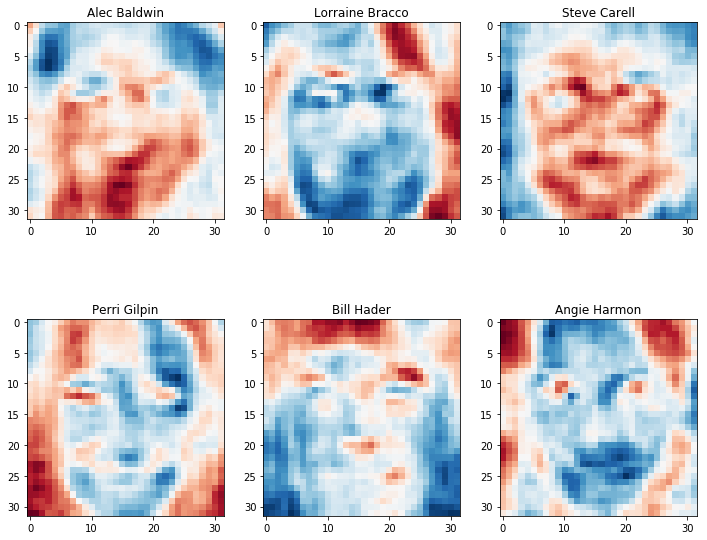
\includegraphics[scale=.55]{pics/6_faces.png}
\end{figure}



\end{homeworkProblem}


\end{document}